
%(BEGIN_QUESTION)
% Copyright 2009, Tony R. Kuphaldt, released under the Creative Commons Attribution License (v 1.0)
% This means you may do almost anything with this work of mine, so long as you give me proper credit

Suppose we are using a control valve to throttle the flow of crude oil through a heater, fired by natural gas burners:

$$\includegraphics[width=15.5cm]{i00793x01.eps}$$

The flow is normally controlled on the basis of the crude oil's exiting temperature from the heater.  In this particular application, should we choose a fail-closed or a fail-open valve?  Why?  Also, if the valve in question is actuated by a pneumatic spring-and-diaphragm assembly, will this be an air-to-close or an air-to-open valve?

Finally, once you have determined the proper failure mode for the valve, determine the proper control action (direct or reverse) for the controller.

\vskip 20pt \vbox{\hrule \hbox{\strut \vrule{} {\bf Suggestions for Socratic discussion} \vrule} \hrule}

\begin{itemize}
\item{} Articulate a strategy for analyzing such systems step-by-step, so that you {\it know} you have arrived at the correct answer(s).
\item{} For those who have studied thermocouple temperature transmitters, determine whether the TT should be configured for {\it upscale} or {\it downscale} burnout.
\end{itemize}

\underbar{file i00793}
%(END_QUESTION)





%(BEGIN_ANSWER)

We should choose a fail-open valve, which would be an air-to-close valve (if pneumatically actuated). If the valve were to fail closed, the heater tubes would overheat, causing a crude oil leak above the natural gas burners, thus causing a large fire.  Failing the valve in the full-open position will actually cool down the heater tubes and prevent a rupture.

However, maximum flow through the heater tubes can cause other problems in the process as well, such as distillation tower flooding.  An alternative solution is to use a fail-closed valve (air-to-open) equipped with minimum-flow stops that prevent the valve from ever going fully closed.

Another alternative plan is to install a manual {\it bypass} valve in parallel with the control valve, then chain-lock that manual valve at some low-flow setting.  This way, when our fail-closed control valve goes fully closed, there is still some minimum amount of crude oil flow through the heater tubes.  If operations personnel ever truly wish to halt flow, they can unlock the manual valve and shut it too.

\vskip 10pt

If the transmitter wires break, the PV signal will fall below zero percent.  This will drive the output of a reverse-acting controller {\it up}, which in this case will drive the control valve shut.  This, clearly, is not the failure mode we intended when specifying an air-to-close valve.

The best fix for this is to configure the temperature transmitter for reverse action, and the controller for direct action.  In other words, an increasing temperature will drive its 4-20 mA signal down.  This way, an open fault in the transmitter wiring will look like a high temperature ($>$ 100\%) to the controller, which being direct-acting will decrease its output and allow the valve to go to its resting (fail-safe) state.

%(END_ANSWER)





%(BEGIN_NOTES)


%INDEX% Final Control Elements, valve: fail safe
%INDEX% Process: crude oil heater (fired)

%(END_NOTES)


